\section{Motivating Examples}


\begin{figure*}[t]
  \centering
  \begin{subfigure}[b]{.3\linewidth}
      \centering
      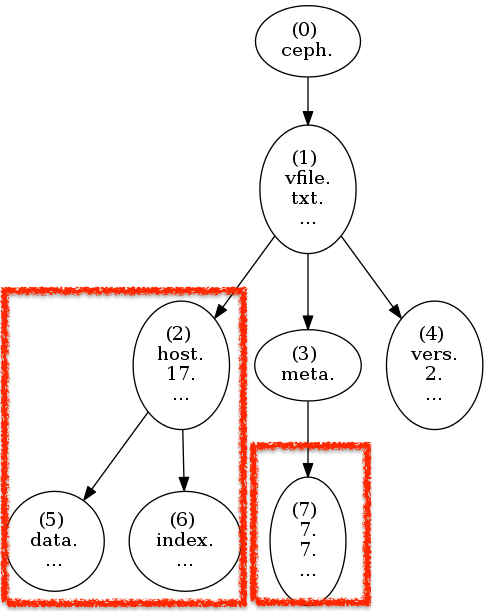
\includegraphics[width=1.0\linewidth]{figures/tree_plfs.png}
      \caption{PLFS} \label{fig:plfs}
  \end{subfigure}
  \begin{subfigure}[b]{.3\linewidth}
      \centering
      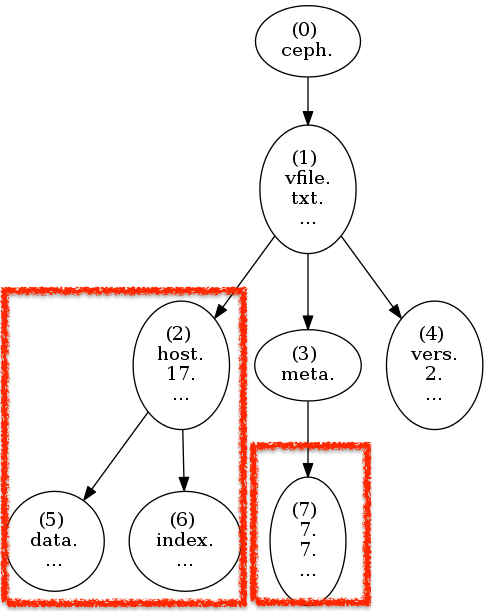
\includegraphics[width=1.0\linewidth]{figures/tree_plfs.png}
      \caption{PLFS} \label{fig:plfs}
  \end{subfigure}
  \begin{subfigure}[b]{.3\linewidth}
      \centering
      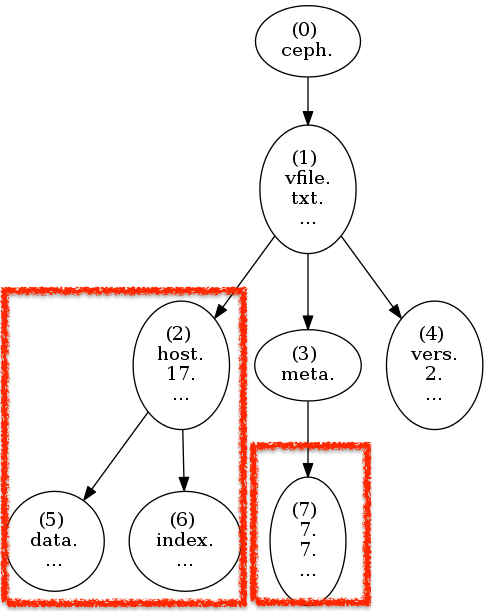
\includegraphics[width=1.0\linewidth]{figures/tree_plfs.png}
      \caption{PLFS} \label{fig:plfs}
  \end{subfigure}
\caption{Namespaces generated by 3 motivating examples.\label{fig:use-cases}}
\end{figure*}

To motivate implied namespaces, we look at the namespaces of 3 applications.
Each is from different domains and this list is not meant to be exhaustive, as
similar organizations exist for many domains, even something as distant as the
mail application on a Mac. For scalability reasons, we focus on large scale
systems in high performance computing (HPC) and high energy physics (HEP).

\subsection{PLFS (HPC)}
\label{sec:plfs}
% What is the problem the authors are trying to solve?
Checkpointing performs small writes to a single shared file but because
filesystems are optimized for large writes, performance is poor. To be
specific, it easier for applications to write checkpoints to a single file with
small, unaligned, writes of varying length varying write (N-1) but
general-purpose distributed file systems are designed for writes to different
files (N-N).

% What is the general problem
The problem is that the application understands the workload but it cannot
communicate a solution to the storages system. The common solution is to add
middleware (i.e. software that sits between the application and the storage
system) to translate the data into a format the storage system performs well
at. In this section, we examine a motivating example
(Section~\ref{sec:motivating-example-plfs}) and a compression technique for that example
use to communicate (Section~\ref{sec:language-patterned-io})
(Section~\ref{sec:adapting-to-the-workload-with-cudele}).  

% What is the problem?
The problem is that the underyling file system cannot keep up with the metadata
load imposed by PLFS. PLFS creates an index entry for every write, which
results in large per-processes tables ~\cite{grider:pc17-diddlings}. This makes
reading or scanning a logical file slow because PLFS must construct a global
index by reading each process's local index. This process incurrs a
\texttt{readdir} and, if the file is open by another process, an additional
\texttt{stat()} because metadata cannot be cached in the
container~\cite{bent_plfs_2009}.

\subsubsection{System Architecture}
%@noah: there is an index because applications do not have regular IO
PLFS~\cite{bent_plfs_2009} solved the checkpoint problem by mapping logical
files to physical files on the underlying file system. The solution targets N-1
strided checkpoints, where many processes write small IOs to offsets in the
same logical file. The key insight of PLFS is that general purpose file systems
perform well for applications that use N-N checkpoints and that the N-1 strided
checkpoint style can be transformed with a thin interposition layer. To map
offsets in the logical file to physical files each process maintains an index
of \{logical offset, physical offset, length, physical block id\}. 

% What is the authors' approach or solution?
PLFS maps an application's preferred data layout into one that the file system
performs well on. Each process appends writes to a different data file in the
hierarchical file system and records an offset and length are recorded in an
index file. Reads aggregate per-process index files into a global index file,
which it uses as lookup table for logical file. 

% Why is it better than the other approaches or solutions?
This solution improves write bandwidth and the single indexing reduces the
number of files in a container. This PLFS layer successfully takes an N-1
checkpoint format and changes the layout and organizes the checkpoints as an
N-N checkpoint directory hierarchy. Each directory represents a node and has
data and indexes (which improve reads). This way, writes are are not small and
interspersed but can be done quickly and effectively in each subdirectory
underneath the checkpoint1 root.

% What other approaches or solutions existed at the time that this work was done?
Checkpointing is the most common way to save the state of the application to
persistent storage for fault tolerance. There are 3 flavors of checkpointing:
N-N (unique files), N-1 (1 file), and N-1 striped (1 file with blocks). LFS
systems (WAFL and Panasas's Object Storage) have a similar approach to PLFS
which reorganizes disk layouts for sequential writing, Berkeley Lab Checkpoint
/ Restart and Condor checkpointing use applications to check node states,
stdchk saves checkpoints in a  diskless cloud, adaptable IO systems
aggressively log and use write-behinds, and Zest uses a manager for each disk
to pull data from distributed queues.

% What was wrong with the other approaches or solutions?
An N-1 checkpoint pattern receives far less bandwidth than an N-N pattern. N-N
applications have more overhead, are harder to manage/archive, are harder to
visualize, and have worse failure recovery (all in 1 file) than N-1 patterns.
Furthermore, N-1 programmers do not want change their code to an N-N
checkpointing scheme and do not want to change their coding style to facilitate
the increased bandwidth. All systems current hybrid systems have drawbacks,
such as a failure to decouple concurrency, storage overhead, the behavior of
HPC parallel applications (utilizing all memory), application modification, and
availability of data.

\subsubsection{Language: Pattern PLFS}
\label{sec:language-patterned-io}

% What other approaches or solutions existed at the time that this work was done?
I/O access patterns are studied extensively and results are integrated into
existing systems. The common checkpointing technique, employed by ADIOS and
PLFS, transform the concurrently written file into exclusively written file
fragments. 

% What was wrong with the other approaches or solutions?
Despite extensive studies on I/O access patterns, current systems do not
dynamically recognize patterns at a fine granularity. Because the PLFS
checkpoint technique makes many small writes, it is either slow (on disk) or
consumes a large amount of space (memory).  

% What is the authors' approach or solution?
The authors present algorithms to discover and replace PLFS metadata. The
system is composed of: 

\begin{itemize}

  \item local per-process metadata: split based on pattern discovering engine
  (get tuples using sliding window)

  \item merge local indices into a single global one per PLFS (check if local
  neighbors abut each other)

\end{itemize}

% Why is it better than the other approaches or solutions?
The authors' algorithms rediscover information as data moves through POSIX. By
dynamically  pattern matching and compression, they are able to reduce latency
and disk/memory usage on reads. 

% How does it perform?
They tested with FS-TEST, MapReplayer, and real applications. In their
experiments, metadata is reduced by several orders of magnitude, write
performance is increased (by 40\%), and reads are increased (by 480\%). 

% Why is this work important?

Discovering structure in unstructured IO is useful for other systems, like
pre-fetching and pre-allocation of blocks in file system or SciHadoop
(metadata/data). This work that these algorithms (applied to compress metadata)
can successfully optimize I/O. 

% 3+ comments/questions
\begin{itemize}

  \item What PLFS structures allow us to to this?

  \item How dependent on workloads are these?

  \item Can this be extended to other file systems?

\end{itemize}

\subsubsection{Namespace Description}

\subsection{ROOT (HEP)}

% the data
The High energy physics (HEP) community uses a framework called ROOT to
manipulate, manage, and visualize data about proton-proton collisions
collected at the large hydron collider. The data is used to re-simulate
phenomena of interest for analysis and there are different types of
reconstructions each with ifferent granularities. The data is organized as
nested and object oriented event data and the length of the runs (and thus
the number of events) are of arbitrary length and type ({\it e.g.},
particle objects, records of low-level detector hit properties).
Reconstruction takes detector conditions ({\it e.g.} alignment, position of
the beam, etc.) as input, which is pulled from remote database.  Data is
streamed from the LHC into large immutable datasets, stored publicly in
data centers around the world.  Physicists search the dataset and download
interesting events, which are stored as ROOT files. 

\subsubsection{System Architecture}

% WHat does ROOT have?
The advantages of the ROOT framework is the ability to (1) read only parts
of the data and (2) easily ingest remote data over the network. The
disadvantage of the ROOT framework and ROOT files have no formal
specification. Much of the development was done at CERN in parallel with
other HPC ventures. As a result, the technology and strategies are similar
to existing systems:

\begin{itemize}
  \item subdirectories within a file, for organization like HDF5
  \item serialization of any type of C++ object, like Python's pickle, but for C++
  \item embedded schema with schema evolution like Avro
  \item columnar storage of large sets of events, like the Dremel/Parquet shredding algorithm (called "splitting" in ROOT)
  \item selective reading, also like Dremel/Parquet (the "prune" feature of SparkSQL DataFrames)
  \item mutable content; a ROOT file is effectively a single-user object database (but without ORM: the data are fundamentally not relational— maybe "document store" would be a better word for what it's doing). Not all operations are guaranteed to be atomic or thread-safe (hence "single-user").
\end{itemize}

% ROOT files
A ROOT file is a list of objects, accessed by consulting metadata in the
header and seeking to a location in the bytestream. Types of objects include: 

\begin{itemize}

  \item TDirectory: collection of TKeys

  \item TKey: object metadata containing name, title, classname, and seek
  position

  \item TTree: table of a collection of events, listed sequentially and stored in a flat namespace

  \item TBranch: data container representing column(s) of TTree

  \item TLeaf: data type description, stored as a special TBranch memeber
  that describes the TBranch's data type

  \item TBasket: byte ranges partitioned by events and indexed by TKeys;
  also the compression, parallelization, and tranfer unit

\end{itemize}

The \texttt{splitlevel} parameter controls the data layout, {\it i.e.}
whether it is organized more closely to rowwise or columnar. Low values
store columns values as tuples in entries ({\it i.e.} \texttt{splitlevel=0}
stores all column values as tuples in each entry) while high values make
the data more columnar-based. Other parameters control the size and shape
of hierarchical structure of the ROOT file include events per file, target
TBasket size, cluster size, compression algorithm and level, and alignment
of objects with disk pages.

\subsubsection{Future integrations with CephFS}

ROOT uses a flat file to describe hierarchical data because there are too many
branches to create a file for each and there is not enough metadata to
reconstruct which branches belong to which events.

Questions: 
- what does MetaData and Events mean? What is the difference!?
- this namespace looks like it only goes one deep... how do I find other TTrees? OR
- is it only the TBranches/tuples/splitting that makes this hierarchical data? 
  - how do we make it look like something a scientist would actually do?

\subsubsection{Namespace Description}

We run ROOT with the following commands to build up the namespace:

TODO visualize the namespace
root -b ./2AC36403-8E7E-E711-A599-02163E01366D.root
.ls
MetaData->Print()

\subsection{SIRIUS (HPC)}
